\documentclass[sigconf,nonacm]{acmart}

\settopmatter{printacmref=false}
\renewcommand\footnotetextcopyrightpermission[1]{}
\pagestyle{plain}

\usepackage{booktabs}
\usepackage{array}
\usepackage{graphicx}
\usepackage{amsmath}
\usepackage{xurl}
\usepackage{placeins}

\title{Parallel Breadth-First Search: GPU Linear Algebra, Graph-First Traversal, and Distributed MPI Partitioning}

\author{Aakaash Nattanmai}
\affiliation{%
  \institution{Cornell University}
  \city{Ithaca}
  \state{NY}
  \country{USA}}
\email{}

\author{Harshaan Chugh}
\affiliation{%
  \institution{Cornell University}
  \city{Ithaca}
  \state{NY}
  \country{USA}}
\email{}

\begin{abstract}
Breadth-first search (BFS) is a core graph primitive, but its irregular
frontiers and skewed memory access patterns make it difficult to optimize on
modern parallel systems. This project compares three BFS design spaces:
linear-algebraic GPU BFS, graph-first direction-optimizing GPU BFS, and
distributed-memory MPI BFS. On a single NVIDIA A100, we implement five
linear-algebraic sparse-matrix-vector-style BFS variants and a graph-first
push/pull traversal. On Perlmutter CPU nodes, we extend the project with 1D
and 2D MPI graph partitioning, bitmap frontier reductions, and SNAP road
network benchmarks. The fastest SpMV-style GPU variant wins on all six
synthetic GPU inputs, with graph-first within 1.14--1.33x on random
sparse/dense graphs but 2.69x slower on the power-law graph. In MPI, 2D
partitioning improves the dense synthetic graph at 16 ranks, while 1D bitmap
frontier reductions are consistently better on sparse road networks up to 64
ranks. These results suggest that no single BFS formulation dominates: the
best design depends on whether memory bandwidth, frontier construction,
communication volume, or graph diameter is the limiting cost.
\end{abstract}

\begin{document}
\maketitle

\section{Introduction}

BFS is a building block for shortest paths, connected components, centrality,
web crawling, and many graph analytics pipelines. It is also a representative
stress test for high-performance computing: each level depends on the previous
frontier, work per vertex is highly irregular, and memory accesses follow graph
structure rather than dense array order. On GPUs, this creates warp divergence,
load imbalance, and atomic update pressure. On distributed-memory systems, it
turns into a communication problem because each frontier may contain vertices
owned by many ranks.

Our project asks how the choice of abstraction affects BFS performance. We
started from the course suggestion to compare a graph-first BFS with a
linear-algebraic formulation inspired by GraphBLAS. We then extended the study
after the poster checkpoint with MPI implementations that compare 1D and 2D
partitioning. Our hypothesis was that linear-algebraic GPU kernels would be
competitive when frontier operations could be expressed as regular sparse row
scans, while graph-first traversal would benefit when frontier sizes were small
enough to avoid scanning most vertices. For MPI, we expected 2D partitioning to
reduce communication at high rank counts, especially on graphs with enough
edges to amortize its extra setup.

The project contributions are:
\begin{itemize}
    \item five CUDA BFS kernels: baseline, warp-cooperative, bitmap,
    push-pull, and fused warp-bitmap;
    \item a CUDA graph-first BFS with top-down push, bottom-up pull, bitmap
    frontiers, and Beamer-style alpha/beta switching;
    \item 1D and 2D MPI BFS implementations with bitmap frontiers,
    bitwise-OR reductions, and SNAP road-network support;
    \item correctness validation against a Python BFS and benchmark results on
    synthetic and real road graphs.
\end{itemize}

\section{Related Work}

Beamer et al. introduced direction-optimizing BFS~\cite{beamer2012}, which
motivates the push/pull split in our graph-first CUDA implementation. In
top-down mode,
frontier vertices push discoveries to neighbors; in bottom-up mode, unvisited
vertices pull by checking whether any neighbor is in the frontier. Merrill et
al.~\cite{merrill2012} showed that GPU BFS needs careful frontier management,
load balancing, and prefix/bitmap techniques to avoid underutilization. Our
warp-cooperative and bitmap variants are simplified experiments in that design
space.

The linear-algebraic framing is motivated by GraphBLAS and related work that
casts graph traversal as sparse linear algebra over semirings~\cite{kepner2016}.
The MPI extension is motivated by distributed sparse matrix and graph
partitioning work, especially 2D sparse matrix distributions used in
CombBLAS~\cite{buluc2011}. Our SNAP road-network inputs follow the SNAP graph
collection~\cite{snap}.

\section{Implementations}

\subsection{Common Graph Representation}

All GPU variants use the same host-side graph loader and CSR representation:
\texttt{row\_ptr[V+1]} and \texttt{col\_idx[E]}. Synthetic graph files are
stored as undirected edge lists and loaded with both directions inserted. The
MPI loader supports both the project \texttt{.edgelist} format and SNAP
\texttt{.txt} files. Each implementation computes integer BFS depths from a
fixed source vertex and can dump full depth vectors for validation.

\subsection{Linear-Algebraic GPU BFS}

The linear-algebraic implementation expresses each BFS level as a masked sparse
matrix-vector operation
\[
    f_{k+1} = (A f_k) \odot \neg v_k,
\]
where $f_k$ is the frontier and $v_k$ is the visited mask. We implemented five
kernel variants.

The \textbf{baseline} assigns one CUDA thread per vertex and scans that row for
any neighbor in the current frontier. \textbf{Warp-cooperative} processing
assigns one warp per row, so high-degree rows are split across 32 lanes and
combined with a warp vote. The \textbf{bitmap} variant compresses the frontier
from one integer per vertex to one bit per vertex, reducing bandwidth and cache
pressure. \textbf{Push-pull} adds a frontier-driven push kernel for small
frontiers and switches to pull when an estimated edge budget crosses a Beamer
threshold. Finally, \textbf{warp-bitmap} combines warp-cooperative row scans
with bitmap frontier checks.

\subsection{Graph-First GPU BFS}

The graph-first CUDA implementation uses frontier queues and bitmap frontiers.
The top-down kernel assigns one thread to each frontier vertex and
uses \texttt{atomicCAS} on \texttt{visited[]} to prevent duplicate discoveries.
The bottom-up kernel assigns one thread to each unvisited vertex and stops as
soon as it finds a neighbor in the frontier bitmap. The host maintains the
frontier size and frontier edge count each level. It switches from top-down to
bottom-up when $m_f > |E|/\alpha$ and switches back when
$|f_k| < |V|/\beta$, using $\alpha=14$ and $\beta=24$ by default.

\subsection{MPI BFS}

The post-poster extension adds two CPU-only MPI BFS implementations. The 1D
version partitions vertices into contiguous row blocks. Each rank scans its
locally owned unvisited vertices using a global frontier bitmap, then contributes
new discoveries through \texttt{MPI\_Allreduce} with \texttt{MPI\_BOR}. The
bitmap representation makes each frontier a fixed-size $|V|/8$ byte buffer and
maps naturally to set union. Early termination is implemented by popcounting the
merged frontier.

The 2D version arranges ranks into a $\sqrt{P}\times\sqrt{P}$ grid and assigns
each rank a block of the adjacency matrix. Each rank extracts the frontier slice
for its column block, scans its local submatrix, and OR-reduces newly discovered
row-block vertices within its process row. For simplicity, the implementation
still keeps a full global frontier and depth vector on each rank and performs a
global OR to assemble the next frontier. This makes the 2D implementation a
useful partitioning experiment, but not a fully memory-minimal distributed BFS.

\section{Cost Model}

BFS performance can be separated into per-level work and per-level
synchronization. On the GPU, a simplified traversal time is
\[
    T_{\mathrm{GPU}} \approx L t_{\mathrm{launch}}
    + \sum_{k=1}^{L} (M_k / B_{\mathrm{mem}} + A_k t_{\mathrm{atomic}}),
\]
where $L$ is the number of BFS levels, $M_k$ is the memory traffic for level
$k$, and $A_k$ is the number of atomic updates. This explains why a chain graph
is slow despite having few edges: it has many levels and very little parallel
work per launch. It also explains why power-law graphs stress graph-first push:
high-degree hubs can create many atomic queue updates in the same level.

For the MPI bitmap BFS, let $W=\lceil |V|/64\rceil$ be the number of 64-bit
bitmap words and $P$ the number of ranks. The 1D implementation performs one
global OR-reduction over $W$ words per level, so an alpha-beta model gives
\[
    T_{\mathrm{1D},k} \approx C_k/P
    + \alpha \log P + 8 W \beta \log P ,
\]
where $C_k$ is local edge-scan work. The 2D prototype adds a row reduction over
$W/\sqrt{P}$ words, but still assembles a full global frontier:
\[
    T_{\mathrm{2D},k} \approx C_k/P
    + \alpha \log \sqrt{P} + 8(W/\sqrt{P})\beta \log \sqrt{P}
    + \alpha \log P + 8W\beta \log P .
\]
Thus 2D can win when the reduced local edge work and row-level collectives
matter, but the current prototype still pays a global-frontier cost. This model
matches the experiments: 2D helps most on the dense synthetic graph and least
on sparse road networks with many low-work levels.

\section{Experimental Methodology}

GPU experiments ran on one NVIDIA A100 on NERSC Perlmutter with
\texttt{CUDA\_VISIBLE\_DEVICES=0}. Timings use CUDA events around the traversal
only, excluding graph load and output. Each reported GPU number is the median
of 10 runs. MPI experiments ran on Perlmutter CPU nodes with 10 trials for
synthetic graphs and 3 trials for SNAP road networks. MPI timings use
\texttt{MPI\_Wtime} around the BFS traversal.

We used six synthetic inputs: medium graphs with $10^3$ vertices and large
graphs with $10^5$ vertices, covering chain, dense random, sparse random, and
power-law structure. We also evaluated SNAP road networks: roadNet-PA,
roadNet-TX, and roadNet-CA. Correctness was checked on tiny graphs against a
Python BFS. For SNAP, we checked that 1D runs with different rank counts and
the 2D implementation produced matching depth vectors on the same source.

\section{GPU Results}

\begin{figure}[t]
    \centering
    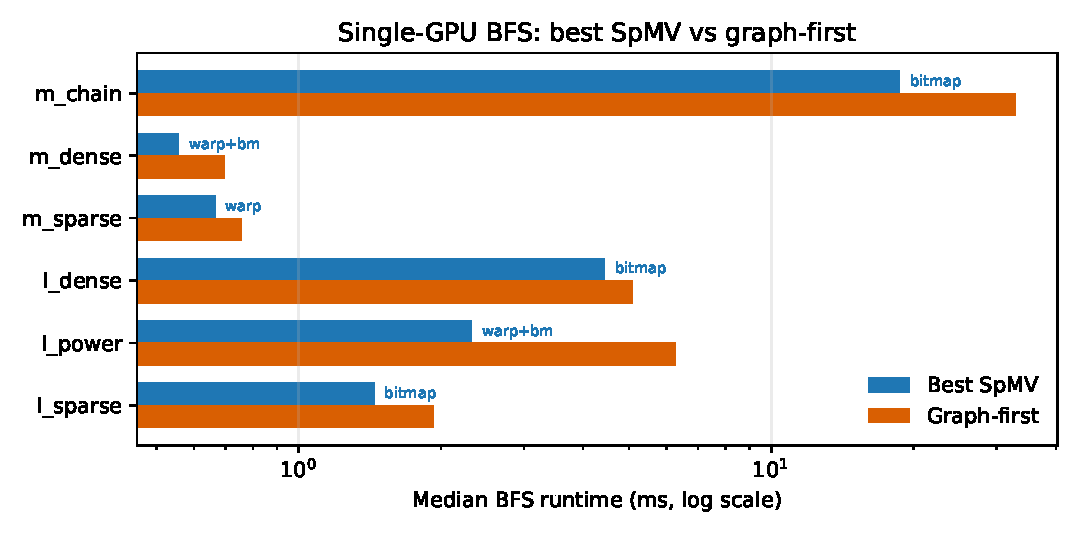
\includegraphics[width=\linewidth]{figures/gpu_head_to_head.pdf}
    \caption{Single-GPU A100 runtime comparison. Each blue bar is the fastest
    linear-algebraic SpMV variant for that graph; orange is graph-first
    direction-optimizing BFS. The x-axis is logarithmic.}
    \Description{Horizontal bar chart comparing best SpMV and graph-first BFS runtimes.}
    \label{fig:gpu}
\end{figure}

\begin{table}[t]
\centering
\caption{Median GPU BFS time in milliseconds. The best SpMV variant is selected
per graph and compared with graph-first direction optimization.}
\label{tab:gpu}
\small
\begin{tabular}{@{}l l r r r@{}}
\toprule
Graph & Best SpMV & SpMV & Graph-first & Ratio \\
\midrule
medium\_chain & bitmap & 18.733 & 32.918 & 1.76x \\
medium\_dense & warpbitmap & 0.557 & 0.697 & 1.25x \\
medium\_sparse & warp & 0.665 & 0.758 & 1.14x \\
large\_dense & bitmap & 4.438 & 5.085 & 1.15x \\
large\_powerlaw & warpbitmap & 2.325 & 6.264 & 2.69x \\
large\_sparse & bitmap & 1.446 & 1.927 & 1.33x \\
\bottomrule
\end{tabular}
\end{table}

Figure~\ref{fig:gpu} and Table~\ref{tab:gpu} show that the best
linear-algebraic variant wins on all six current GPU inputs. This does not mean
that a generic SpMV formulation is always faster; rather, it reflects the
particular costs of our graph-first implementation. Graph-first must construct
new queues, maintain queue and bitmap representations, and use atomics during
push. On random sparse and dense graphs, the gap is modest: 1.14--1.33x on
medium/large sparse and large dense. The large power-law graph is the hardest
case for graph-first because hub-heavy frontiers amplify queue and atomic
overhead. The chain graph is pathological for both paradigms because the BFS
depth is 999, forcing many sequential kernel launches with little parallel work
per level.

The SpMV variants also show that optimizations are topology-dependent. Bitmap
frontiers improve bandwidth pressure on large dense and sparse graphs. The
warp-bitmap fusion is best on the large power-law graph, where high-degree hubs
benefit from cooperative row scanning. Push-pull is not universally helpful in
the SpMV code because its switching heuristic uses an average-degree estimate;
on some inputs, the extra bookkeeping outweighs the saved work.

\FloatBarrier
\section{MPI Results}

\begin{figure}[t]
    \centering
    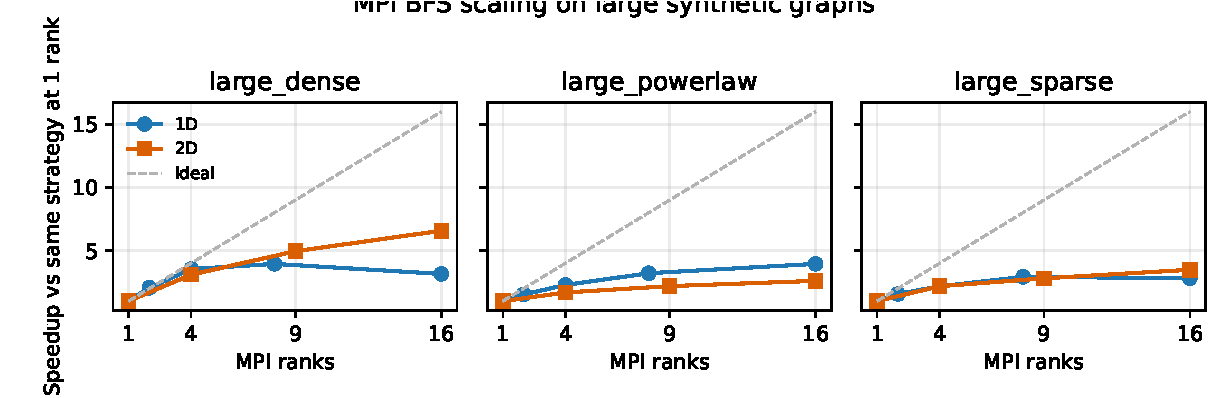
\includegraphics[width=\linewidth]{figures/mpi_synthetic_speedup.pdf}
    \caption{MPI speedup on the large synthetic graphs. Speedup is normalized
    against the same strategy at one rank.}
    \Description{Three panel line chart of MPI speedup for large dense, power-law, and sparse graphs.}
    \label{fig:mpi-synth}
\end{figure}

\begin{table}[t]
\centering
\caption{Large synthetic MPI results at 16 ranks. Speedup is relative to the
same strategy at one rank.}
\label{tab:mpi-large}
\small
\begin{tabular}{@{}l r r r r@{}}
\toprule
Graph & 1D time & 1D speedup & 2D time & 2D speedup \\
\midrule
large\_dense & 0.006686 & 3.15x & 0.003220 & 6.57x \\
large\_powerlaw & 0.001485 & 3.95x & 0.002615 & 2.60x \\
large\_sparse & 0.003157 & 2.82x & 0.003262 & 3.48x \\
\bottomrule
\end{tabular}
\end{table}

\begin{figure}[t]
    \centering
    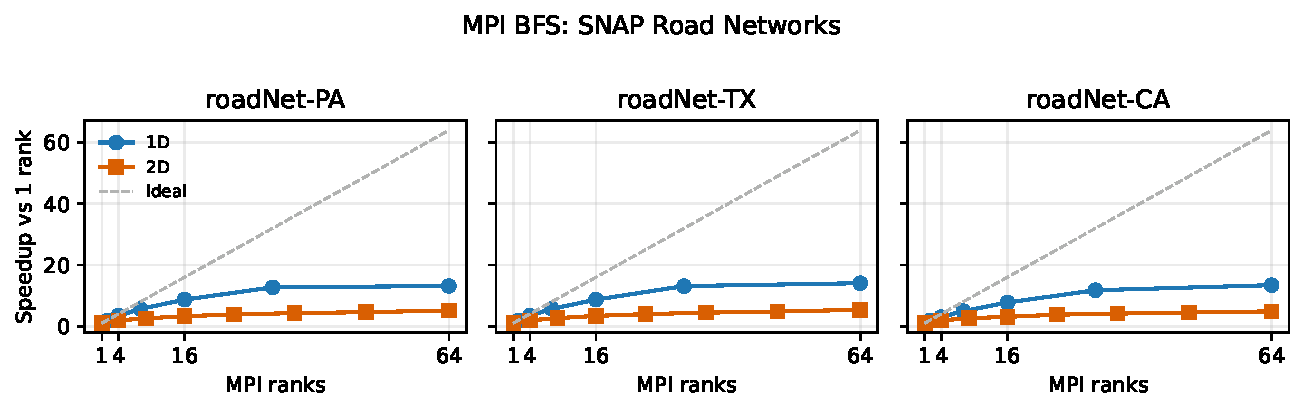
\includegraphics[width=\linewidth]{figures/mpi_snap_speedup.pdf}
    \caption{MPI speedup on SNAP road networks. 1D partitioning scales better
    than the current 2D prototype on these sparse high-diameter road graphs.}
    \Description{Three panel line chart of MPI speedup for SNAP road networks.}
    \label{fig:mpi-snap}
\end{figure}

\begin{table}[t]
\centering
\caption{SNAP road-network MPI results at 64 ranks. 1D speedup is relative to
the 1D one-rank runtime.}
\label{tab:mpi-snap}
\small
\begin{tabular}{@{}l r r r@{}}
\toprule
Graph & 1D 64-rank time & 1D speedup & 2D 64-rank time \\
\midrule
roadNet-PA & 0.243842 & 13.14x & 0.863500 \\
roadNet-TX & 0.383658 & 14.06x & 1.390648 \\
roadNet-CA & 0.412492 & 13.41x & 1.611111 \\
\bottomrule
\end{tabular}
\end{table}

The MPI results answer a different question than the GPU results: how BFS
partitioning interacts with communication. On the large dense synthetic graph,
2D partitioning has the best high-rank result, reaching 0.003220 s at 16 ranks
compared with 0.006686 s for 1D. This supports the expected advantage of 2D
partitioning when enough edges exist to amortize submatrix setup and when row
reductions reduce per-rank work.

The power-law and sparse synthetic graphs favor 1D. On large power-law, 1D
improves from 0.005864 s at one rank to 0.001485 s at 16 ranks, while 2D
improves from 0.006811 s to 0.002615 s. On large sparse, the two strategies are
close at 16 ranks. These results suggest that our 2D implementation is most
useful when edge work is high; otherwise, the global-frontier simplification
and extra reductions dominate.

SNAP road networks strengthen this conclusion. Table~\ref{tab:mpi-snap} shows
that 1D reaches roughly 13--14x speedup at 64 ranks on all three road networks.
For roadNet-CA, 1D improves from 5.53 s at one rank to 0.41 s at 64 ranks,
while 2D improves from 7.82 s to 1.61 s. 1D also wins on roadNet-PA and
roadNet-TX at all tested rank counts.
Road graphs have low average degree and high diameter, so each level has
relatively little edge work and many synchronization rounds. The fixed global
bitmap reduction in 1D is simple and efficient enough that the current 2D
prototype's extra communication is not recovered.

\FloatBarrier
\section{Validation and Reproducibility}

Correctness was checked in three ways. First, all tiny edgelist graphs were
validated against \texttt{test-graphs/validate\_bfs.py}. Second, the GPU
benchmark harness can pass \texttt{--dump} to emit one depth per vertex for
comparison. Third, the MPI SNAP tests compared depth vectors across 1D and 2D
executions rather than checking only aggregate counts. This is important
because two BFS implementations can report the same number of reachable
vertices while still disagreeing on levels.

All benchmark commands are scripted. GPU experiments use the Python benchmark
driver in \texttt{scripts/}; MPI experiments use the Slurm batch scripts in the
same directory. The report figures are regenerated by
\texttt{scripts/plot\_report\_results.py} from committed CSV files, which keeps
the PDF plots tied to the raw data. Build instructions and result paths are
documented in the repository README.

\FloatBarrier
\section{Discussion}

The main lesson is that BFS optimizations are strongly graph- and
architecture-dependent. On a single GPU, dense bitmap and warp-cooperative
frontier representations are valuable because they reduce bandwidth and load
imbalance. However, a graph-first implementation needs careful queue
construction to compete with row-scan SpMV kernels. In distributed-memory MPI,
the same BFS problem becomes a frontier communication problem: bitmap OR
reductions are simple and robust, while 2D partitioning only helps when
communication reduction exceeds the cost of additional coordination.

Our study has limitations. The GPU implementations are hand-written CUDA
kernels rather than cuGraph or a production GraphBLAS backend. The MPI
implementations are CPU-only and load graphs by broadcasting edge arrays from
rank 0, which is adequate for our project graphs but not scalable to
Graph500-sized inputs. The 2D MPI implementation keeps global frontier and depth
arrays for simplicity, so it tests a 2D work partition but not the full memory
savings of a distributed 2D BFS. Finally, GPU and MPI timings should not be
interpreted as direct hardware comparisons; they answer different design
questions.

\section{Future Work}

The most immediate improvement is to make the graph-first GPU BFS more
competitive by reducing queue construction overhead. A warp-aggregated push
kernel could reserve queue slots per warp rather than per discovered vertex,
reducing atomic contention on power-law graphs. For the SpMV code, the
push-pull heuristic should use the actual frontier edge count rather than an
average-degree estimate, matching the graph-first driver.

For MPI, a stronger 2D implementation would avoid storing the full frontier on
every rank. The diagonal owner of each column block should broadcast frontier
slices down process columns, and row owners should assemble only their
partition of the next frontier. This would better realize the
$O(\sqrt{P})$ communication model. A follow-up experiment should also include
weak scaling on generated RMAT graphs and compare with a tuned distributed
GraphBLAS implementation.

\section{Conclusion}

We implemented and evaluated BFS across two parallel settings. On one A100,
the fastest SpMV-style CUDA kernel outperformed our graph-first traversal on
all current synthetic inputs, though graph-first remained close on random
sparse/dense graphs. After the poster checkpoint, the MPI extension added a
distributed-memory perspective: 2D partitioning improved dense synthetic graphs
at higher rank counts, while 1D bitmap reductions were stronger on sparse road
networks. Together, these experiments show why BFS remains a useful benchmark
for parallel computing: the best algorithm is not simply the one with the most
parallelism, but the one that best matches frontier structure to the memory and
communication costs of the target machine.

\begin{acks}
Experiments were run on NERSC Perlmutter. Source code, scripts, and benchmark
outputs are available at \url{https://github.com/Harshaan-Chugh/parallel-bfs}.
\end{acks}

\begin{thebibliography}{9}

\bibitem{beamer2012}
S. Beamer, K. Asanovic, and D. Patterson.
\newblock Direction-optimizing breadth-first search.
\newblock In \emph{SC '12: Proceedings of the International Conference on High
Performance Computing, Networking, Storage and Analysis}, 2012.

\bibitem{merrill2012}
D. Merrill, M. Garland, and A. Grimshaw.
\newblock Scalable GPU graph traversal.
\newblock In \emph{PPoPP '12}, 2012.

\bibitem{kepner2016}
J. Kepner, P. Aaltonen, D. Bader, A. Buluc, F. Franchetti, J. Gilbert,
D. Hutchison, M. Kumar, A. Lumsdaine, H. Meyerhenke, S. McMillan,
J. Moreira, J. Owens, C. Yang, M. Zalewski, and T. Mattson.
\newblock Mathematical foundations of the GraphBLAS.
\newblock In \emph{IEEE HPEC}, 2016.

\bibitem{buluc2011}
A. Buluc and J. R. Gilbert.
\newblock The Combinatorial BLAS: Design, implementation, and applications.
\newblock \emph{International Journal of High Performance Computing
Applications}, 25(4), 2011.

\bibitem{snap}
J. Leskovec and A. Krevl.
\newblock SNAP datasets: Stanford large network dataset collection.
\newblock \url{https://snap.stanford.edu/data/}, 2014.

\bibitem{gap}
S. Beamer, K. Asanovic, and D. Patterson.
\newblock The GAP benchmark suite.
\newblock \emph{arXiv:1508.03619}, 2015.

\end{thebibliography}

\end{document}
